\documentclass[answers]{exam}
\usepackage{../HT2024}
\usepackage{graphicx}
\graphicspath{ {./images/} }

\title{Dynamics -- Sheet 8}
\author{YOUR NAME HERE :)}
\date{Hilary Term 2024}
% Accurate as of 05/07/2024


\begin{document}
\maketitle
\begin{questions}

\question%1
\begin{parts}
\part%1a
Consider a rigid body that is rotating about a general point $O$ that is fixed both in the body and fixed in an inertial frame. Starting from the point particle model of a rigid body, show that its kinetic energy is \[
	T \equiv \sum_{I=1}^{N} \frac{1}{2} m_{I}|\dot{\mathbf{r}}_{I}|^{2}=\frac{1}{2} \sum_{i, j=1}^{3} \mathcal{I}_{i j}^{(O)} \omega_{i} \omega_{j},
\] where $\mathcal{I}^{(O)}$ is the inertia tensor of the body about $O$, and $\boldsymbol{\omega}$ is its angular velocity. [\emph{Hint}: You might find the vector identity $|\mathbf{a} \wedge \mathbf{b}|^{2}=|\mathbf{a}|^{2}|\mathbf{b}|^{2}-(\mathbf{a} \cdot \mathbf{b})^{2}$ helpful.]

\part%1b
Using the result in part (a), hence show that the kinetic energy of the heavy pendulum, considered at the end of section 8.3 of the lecture notes, is \[
	T=\frac{1}{6} M l^{2} \dot{\theta}^{2}.
\] Here recall that $\theta$ is the angle the pendulum makes with the downward vertical, and the pendulum has length $l$ and mass $M$.

\part%1c
Given that the potential energy is $V=M g Z_{G}$, where $Z_{G}$ is the height of the centre of mass of the pendulum, hence write down the total energy $E=T+V$. Show that conservation of $E$ is implied by the equation of motion (8.47) derived in the lecture notes.
\end{parts}



\question%2
A smooth straight wire rotates with constant angular speed $\omega$ about the vertical axis through a fixed point $O$ on the wire, and the angle between the wire and the upward vertical is constant and equal to $\alpha$, where $0<\alpha<\pi / 2$. A bead of mass $m$ is free to slide on the wire.
\begin{parts}
\part%2a
Starting from the general form of Newton's second law in a rotating frame, show that \[
	m\left(\frac{\mathrm{d}^{2} \mathbf{r}}{\mathrm{d} t^{2}}\right)_{\mathcal{S}}=\mathbf{N}-m g \mathbf{k}-2 m \omega \mathbf{k} \wedge\left(\frac{\mathrm{d} \mathbf{r}}{\mathrm{d} t}\right)_{\mathcal{S}}-m \omega^{2} \mathbf{k} \wedge(\mathbf{k} \wedge \mathbf{r})
\] where $\mathbf{r}(t)$ is the position of the bead in the frame $\mathcal{S}$ that rotates with the wire, $\mathbf{k}$ is a unit vector pointing vertically, and $\mathbf{N}$ is the normal reaction of the wire.

\part%2b
Hence show that $z(t)$, the height of the bead above $O$, satisfies the equation \[
	\ddot{z}-\left(\omega^{2} \sin ^{2} \alpha\right) z=-g \cos ^{2} \alpha .
\] Show that an equilibrium point for the bead exists, and determine its stability.
\end{parts}



\question%3
A bead $P$ of mass $m$ slides on a smooth circular wire of radius $a$ and centre $C$. The wire lies in a horizontal plane and is forced to rotate at a constant angular speed $\omega$ about the vertical axis through a fixed point $O$ in the plane of the wire. The distance from $O$ to $C$ is constant and equal to $b$. Let $\theta$ be the angle that the line joining the centre $C$ to the bead makes with the diameter through $O$. (See the figure below.)
\begin{center}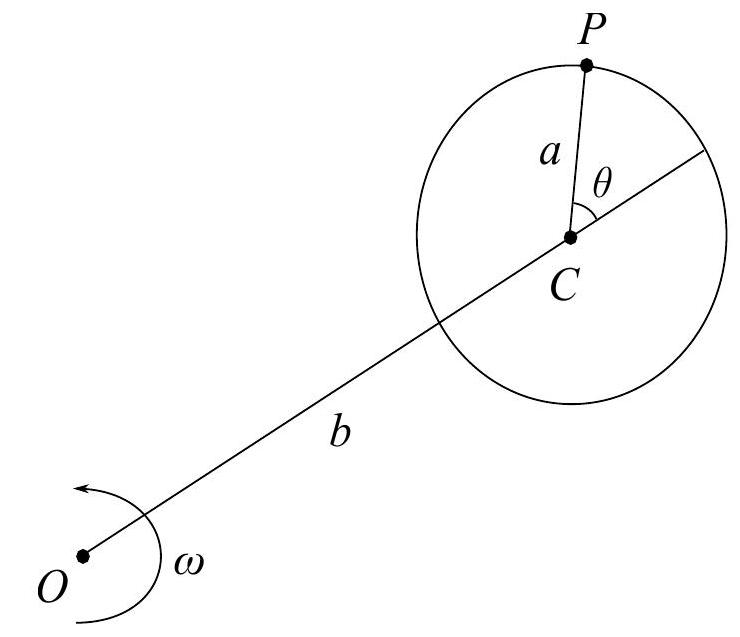
\includegraphics[width=7cm]{sheet 8 diagram}\end{center}
\begin{parts}
\part%3a
Show that the position of the bead may be written as \[
	\mathbf{r}=(b+a \cos \theta) \mathbf{e}_{1}+a \sin \theta \mathbf{e}_{2},
\] where $\mathbf{e}_{i}, i=1,2,3$, are an orthonormal basis for a frame that rotates with the wire.

\part%3b
Using Newton's second law in this rotating frame, hence show that \[
 	\ddot{\theta}+\frac{b}{a} \omega^{2} \sin \theta=0.
\]

\part%3c
Show that the bead can remain in equilibrium relative to the wire at two points. Decide whether these positions of equilibrium are stable or unstable.
\end{parts}



\question%4
(\emph{Optional}) Consider (again) dropping a particle from the top of a tower, of height $h$ above the ground, at time $t=0$. Use a reference frame $\mathcal{S}$ fixed to the surface of the Earth with $\mathbf{e}_{1}$ is a unit vector pointing North, $\mathbf{e}_{2}$ is a unit vector pointing West, and $\mathbf{e}_{3}$ is a unit vector pointing upwards. The origin of this frame is at a latitude $\theta$ on the surface of the Earth and hence the angular velocity of the Earth is given by $\boldsymbol{\omega}=\omega \cos \theta \mathbf{e}_{1}+\omega \sin \theta \mathbf{e}_{3}$, where $\omega=2 \pi /[1$ day $]$.
\begin{parts}
\part%4a
Including only the effects of a uniform gravitational field and the Coriolis force, show that Newton's second law in the frame $\mathcal{S}$ implies \[
	\ddot{\mathbf{r}} \simeq-g \mathbf{e}_{3}+2 g t \boldsymbol{\omega} \wedge \mathbf{e}_{3},
\] where we have assumed that terms of order $\omega^{2}$ are negligible.

\part%4b
Hence show that the trajectory of the particle is given by \[
	\mathbf{r} \simeq\left(h-\frac{1}{2} g t^{2}\right) \mathbf{e}_{3}-\frac{1}{3} \omega g t^{3} \cos \theta \mathbf{e}_{2},
\] and that it lands a distance $d$ to the East of the tower, where \[
	d=\frac{1}{3} \omega \sqrt{\frac{8 h^{3}}{g}} \cos \theta
\]
\end{parts}

\end{questions}

\end{document}
